%%
%% User Guide
%%

%%%%%%%%%%%%%%%%%%%%%%%%%%%%%%%%%%%%%%%%%%%%%%%%%%%%%%%%%%%%%%%%%%%%%%%%%%%%%%%%
\chapter{User Guide}
%%%%%%%%%%%%%%%%%%%%%%%%%%%%%%%%%%%%%%%%%%%%%%%%%%%%%%%%%%%%%%%%%%%%%%%%%%%%%%%%


%%%%%%%%%%%%%%%%%%%%%%%%%%%%%%%%%%%%%%%%%%%%%%%%%%%%%%%%%%%%%%%%%%%%%%%%%%%%%%%%
\section{\qsimavr User Guide}
%%%%%%%%%%%%%%%%%%%%%%%%%%%%%%%%%%%%%%%%%%%%%%%%%%%%%%%%%%%%%%%%%%%%%%%%%%%%%%%%

Within this guide, we will assume the use of firmware compiled for the
\verb|atmega1280| with a frequency of 16 \ac{MHz}\footnote{
%
These are the default settings.
%
}. After starting \qsimavr, you are presented with a screen which should look
somewhat similar to figure \ref{fig:qsimavr}.

\begin{figure}[ht]
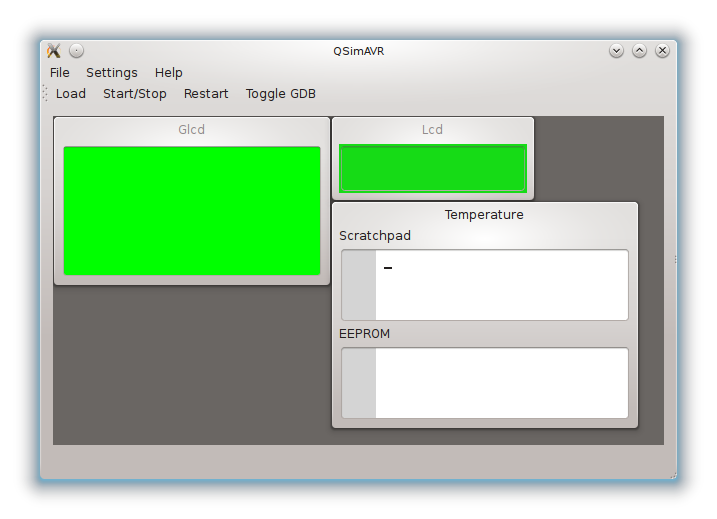
\includegraphics[width=\textwidth]{images/qsimavr}
\caption{\qsimavr}
\label{fig:qsimavr}
\end{figure}

Trace and error output, as well as \simavr messages are printed directly to the
console. \ac{VCD} files are saved into the current working directory.

Loaded components can be configured in the \emph{Settings} menu. Currently,
possible options include enabling or disabling a component and toggling \ac{VCD}
traces.

A firmware file may be loaded by either pressing \emph{Load} in the toolbar,
selecting \emph{Load Firmware...} in the \emph{File} menu, or clicking on one of
the recently loaded files listed in the \emph{File} menu. Simulation starts
automatically once the firmware file has been loaded successfully.

The current simulation state is displayed in the lower left of the status bar
once a firmware file has been loaded.

For debugging (also see \ref{section:debugging}), \ac{GDB} support must be enabled
by clicking the \emph{Toggle \ac{GDB}} button in the toolbar. If a simulation is
currently in progress, execution is halted (note the change in simulation state);
otherwise the \ac{CPU} will be paused once the next firmware file has been loaded
or the simulation is restarted.

Once running, it is possible to pause and unpause the simulation by pressing the
\emph{Start/Stop} button in the toolbar, or restarting it by pressing
\emph{Restart}.

%%%%%%%%%%%%%%%%%%%%%%%%%%%%%%%%%%%%%%%%%%%%%%%%%%%%%%%%%%%%%%%%%%%%%%%%%%%%%%%%
\section{Debugging with \simavr and \ac{GDB}} \label{section:debugging}
%%%%%%%%%%%%%%%%%%%%%%%%%%%%%%%%%%%%%%%%%%%%%%%%%%%%%%%%%%%%%%%%%%%%%%%%%%%%%%%%

% Mention how debugging with qsimavr is exactly the same.
